%\documentclass[journal]{IEEEtran}
\documentclass[10pt,a4paper]{article}
\usepackage{times}
\usepackage{bm,bbm}
\usepackage{amsmath,amssymb}
\usepackage{graphicx,subfigure}
\usepackage{url}
\usepackage{units}
\usepackage{cite,balance}
\usepackage{comment}
\usepackage{multirow}
\usepackage{booktabs}
\usepackage{microtype}
\usepackage{siunitx}
\usepackage{color}
\usepackage{enumerate}

\usepackage{geometry}
\geometry{
	a4paper,
	total={170mm,257mm},
	left=1cm,right=1cm,
	top=1cm,bottom=1.5cm
}



\usepackage[normalem]{ulem} %%%% para tachar texto

\newtheorem{definition}{Definition}
\newtheorem{proposition}{Proposition}
\newcommand{\at}[2][]{#1|_{#2}}

\title{Comparison of methodologies}
\date{}


\begin{document}

\maketitle

\section{Some considerations}
\begin{enumerate}[a)]
	\item $L=3$ case was consdered.
	\item All the optimizations were perfomed by L-BFGS-B version of the Broyden-Fletcher-Goldfarb-Shanno method. We use moment estimator as initial point when it can be found, otherwise $\alpha=-1.5$ was used.
	\item The previous methodology consist in:
	\begin{enumerate}[i)]
		\item Generate $Z_1,\ldots,Z_n$ ramdom variables from a $\mathcal G_I^0(-\alpha,-\alpha-1)$ where $-\alpha>0$ and $E(Z)=1$.
		\item Estimate $Z_i$ distribution with kernel estimation using kernel $K$ ($\widehat f_{\text{\tiny{K}}}(z)$).
		\item Find $\widehat{\alpha}_{\text{\tiny{K}}}= \arg\min_{\alpha} d_{\text{T}}\big(f_{\mathcal{G}^{0}}(-\alpha,\gamma^*, L ), \widehat f_{\text{\tiny{Z,K}}}(z)\big)$ where $\gamma^*=-\alpha-1$.
	\end{enumerate}
	\item The current methodology consist in:
	\begin{enumerate}[i)]
		\item Generate $Z_1,\ldots,Z_n$ ramdom variables from a $\mathcal G_I^0(\alpha,\gamma)$ where $-\alpha>0 \text{, } \gamma>0$.
		\item Define random variables $X_i=\dfrac{Z_i}{\overline{Z}}$.
		\item Estimate $X_i$ distribution with kernel estimation using kernel $K$ ($\widehat f_{\text{\tiny{X,K}}}$).
		\item Find $\widehat{\alpha}_{\text{\tiny{K}}}= \arg\min_{\alpha} d_{\text{T}}\big(f_{\mathcal{G}^{0}}(-\alpha,\gamma^*, L ), \widehat f_{\text{\tiny{X,K}}}\big)$ where $\gamma^*=-\alpha-1$.
	\end{enumerate}
	\item $\widehat f_{\text{\tiny{K}}}$ was performed renormalization the Gamma kernel estimator. 
\end{enumerate}  

\vspace{0.5cm}

\section{Percentage of non-convergence cases }

\vspace{0.5cm}

\begin{minipage}{0.5\linewidth}
\center{\subsubsection*{Previous methodology}}
\begin{tabular}{rrrrr}
	\toprule
	$\alpha$ & $n$ & $\widehat{\alpha}_{\text{ML}}$ & $\widehat{\alpha}_{\Gamma}$ & $\widehat{\alpha}_{\text{LC}}$\\  
	\midrule
	\multirow{5 }{*}{$-1.5$}
	& 9 & 0.0 & 0.0 & 2.8 \\ 
	& 25 & 0.0 & 0.0 & 0.2 \\ 
	& 49 & 0.0 & 0.0 & 0.0 \\ 
	& 81 & 0.0 & 0.0 & 0.0 \\ 
	& 121 & 0.0 & 0.0 & 0.0 \\  
	\midrule
	\multirow{5 }{*}{$-3$}
	& 9 & 13.0 & 5.2 & 28.4 \\ 
	& 25 & 1.0 & 0.2 & 11.4 \\ 
	& 49 & 0.2 & 0.0 & 3.8 \\ 
	& 81 & 0.0 & 0.0 & 2.4 \\ 
	& 121 & 0.0 & 0.0 & 0.2 \\    
	\midrule
	\multirow{5 }{*}{$-5$}
	& 9 & 26.8 & 9.6 & 35.2 \\ 
	& 25 & 10.0 & 3.4 & 28.6 \\ 
	& 49 & 3.4 & 1.4 & 18.6 \\ 
	& 81 & 1.2 & 0.4 & 15.8 \\ 
	& 121 & 0.4 & 0.0 & 9.6 \\   
	\midrule
	\multirow{5 }{*}{$-8$}
	& 9 & 39.6 & 16.6 & 44.2 \\ 
	& 25 & 28.6 & 9.0 & 36.4 \\ 
	& 49 & 18.4 & 5.0 & 31.6 \\ 
	& 81 & 12.0 & 4.4 & 27.2 \\ 
	& 121 & 5.8 & 1.8 & 24.6 \\ 
	\bottomrule
\end{tabular}
\end{minipage}
\;
\begin{minipage}{0.5\linewidth}
	\center{\subsubsection*{Current methodology}}
	\begin{tabular}{rrrrr}
	\toprule
	$\alpha$ & $n$ & $\widehat{\alpha}_{\text{ML}}$ & $\widehat{\alpha}_{\Gamma}$ & $\widehat{\alpha}_{\text{LC}}$\\  
	\midrule
	\multirow{5 }{*}{$-1.5$}
	& 9 & 9.4 & 3.0 & 6.0 \\ 
	& 25 & 0.2 & 0.0 & 0.4 \\ 
	& 49 & 0.0 & 0.0 & 0.0 \\ 
	& 81 & 0.0 & 0.0 & 0.0 \\ 
	& 121 & 0.0 & 0.0 & 0.0 \\  
	\midrule
	\multirow{5 }{*}{$-3$} 
	& 9 & 26.2 & 9.6 & 24.6 \\ 
	& 25 & 4.0 & 0.8 & 4.8 \\ 
	& 49 & 1.0 & 0.2 & 1.0 \\ 
	& 81 & 0.0 & 0.0 & 0.0 \\ 
	& 121 & 0.0 & 0.0 & 0.0 \\	  
	\midrule
	\multirow{5 }{*}{$-5$} 
	& 9 & 41.0 & 14.4 & 39.8 \\ 
	& 25 & 17.4 & 4.0 & 17.6 \\ 
	& 49 & 6.6 & 2.0 & 8.6 \\ 
	& 81 & 1.8 & 0.8 & 2.6 \\ 
	& 121 & 0.6 & 0.0 & 0.6 \\   
	\midrule
	\multirow{5 }{*}{$-8$} 
	& 9 & 53.0 & 21.6 & 52.6 \\ 
	& 25 & 37.0 & 11.4 & 35.2 \\ 
	& 49 & 23.4 & 7.2 & 23.6 \\ 
	& 81 & 16.6 & 4.6 & 15.8 \\ 
	& 121 & 8.4 & 2.8 & 8.2 \\ 
	\bottomrule
\end{tabular}
\end{minipage}

\vspace{1cm}
\section{Bias considering the cases where each estimator converges}

\vspace{1cm}

\begin{minipage}{0.5\linewidth}
\center{\subsubsection*{Previous methodology}}
\begin{tabular}{rrrrr}
	\toprule
	$\alpha$ & $n$ & $\widehat{\alpha}_{\text{ML}}$ & $\widehat{\alpha}_{\Gamma}$ & $\widehat{\alpha}_{\text{LC}}$\\  
	\midrule
	\multirow{5 }{*}{$-1.5$}
	& 9 & -0.172 & -0.183 & -0.242 \\ 
	& 25 & -0.050 & -0.058 & -0.101 \\ 
	& 49 & -0.030 & -0.035 & -0.040 \\ 
	& 81 & -0.025 & -0.036 & -0.032 \\ 
	& 121 & -0.013 & -0.041 & -0.016 \\ 	
	\midrule
	\multirow{5 }{*}{$-3$}
	& 9 & -0.687 & -0.652 & 0.674 \\ 
	& 25 & -0.784 & -0.338 & -0.157 \\ 
	& 49 & -0.348 & -0.014 & -0.306 \\ 
	& 81 & -0.172 & 0.079 & -0.458 \\ 
	& 121 & -0.113 & 0.117 & -0.286 \\ 	
	\midrule
	\multirow{5 }{*}{$-5$} 
	& 9 & -0.088 & 0.084 & 2.309 \\ 
	& 25 & -0.962 & 0.225 & 1.475 \\ 
	& 49 & -0.902 & 0.362 & 0.670 \\ 
	& 81 & -0.674 & 0.318 & 0.222 \\ 
	& 121 & -0.410 & 0.360 & 0.034 \\ 
	\midrule
	\multirow{5 }{*}{$-8$} 	
	& 9 & 2.072 & 2.346 & 5.439 \\ 	
	& 25 & 0.384 & 1.787 & 4.407 \\ 
	& 49 & -0.150 & 1.410 & 3.732 \\ 
	& 81 & -0.650 & 1.260 & 2.649 \\ 
	& 121 & -0.622 & 1.062 & 2.361 \\ 
	\bottomrule
\end{tabular}
\end{minipage}
\;
\begin{minipage}{0.5\linewidth}
\center{\subsubsection*{Current methodology}}
\begin{tabular}{rrrrr}
	\toprule
	$\alpha$ & $n$ & $\widehat{\alpha}_{\text{ML}}$ & $\widehat{\alpha}_{\Gamma}$ & $\widehat{\alpha}_{\text{LC}}$\\  
	\midrule
	\multirow{5 }{*}{$-1.5$} 
	& 9 & -1.352 & -1.367 & -1.512 \\ 
	& 25 & -0.571 & -0.510 & -0.673 \\ 
	& 49 & -0.331 & -0.301 & -0.406 \\ 
	& 81 & -0.216 & -0.195 & -0.275 \\ 
	& 121 & -0.179 & -0.175 & -0.226 \\ 
	\midrule
	\multirow{5 }{*}{$-3$}
	& 9 & -1.285 & -1.304 & -0.456 \\ 
	& 25 & -1.638 & -0.799 & -1.378 \\ 
	& 49 & -0.732 & -0.279 & -0.754 \\ 
	& 81 & -0.438 & -0.082 & -0.494 \\ 
	& 121 & -0.252 & 0.028 & -0.287 \\ 
	\midrule
	\multirow{5 }{*}{$-5$}
	& 9 & -0.851 & -0.383 & 1.436 \\ 
	& 25 & -1.650 & -0.234 & -0.429 \\ 
	& 49 & -1.293 & 0.021 & -0.629 \\ 
	& 81 & -1.178 & 0.010 & -1.033 \\ 
	& 121 & -0.643 & 0.252 & -0.643 \\
	\midrule
	\multirow{5 }{*}{$-8$} 
	& 9 & 1.758 & 1.703 & 4.978 \\ 
	& 25 & -0.195 & 1.452 & 2.706 \\ 
	& 49 & -0.475 & 1.202 & 1.510 \\ 
	& 81 & -0.840 & 0.924 & 0.550 \\ 
	& 121 & -0.778 & 0.947 & -0.093 \\ 
	\bottomrule
\end{tabular}
\end{minipage}

\vspace{1cm}

\section{Mean Squared Error considering the cases where each estimator converges}

\vspace{1cm}

\begin{minipage}{0.5\linewidth}
\center{\subsubsection*{Previous methodology}}
\begin{tabular}{rrrrr}
	\toprule
	$\alpha$ & $n$ & $\widehat{\alpha}_{\text{ML}}$ & $\widehat{\alpha}_{\Gamma}$ & $\widehat{\alpha}_{\text{LC}}$\\
	\midrule
	\multirow{5 }{*}{$-1.5$}
	& 9 & 0.469 & 0.407 & 1.982 \\ 
	& 25 & 0.050 & 0.070 & 0.219 \\ 
	& 49 & 0.020 & 0.034 & 0.043 \\ 
	& 81 & 0.012 & 0.024 & 0.020 \\ 
	& 121 & 0.007 & 0.024 & 0.011 \\
	\midrule
	\multirow{5 }{*}{$-3$}
	& 9 & 6.174 & 5.873 & 8.042 \\ 
	& 25 & 5.869 & 3.542 & 6.937 \\ 
	& 49 & 1.774 & 0.928 & 4.313 \\ 
	& 81 & 0.565 & 0.397 & 3.702 \\ 
	& 121 & 0.375 & 0.239 & 1.767 \\
	\midrule
	\multirow{5 }{*}{$-5$} 
	& 9 & 12.030 & 11.348 & 16.348 \\ 
	& 25 & 11.523 & 6.506 & 15.296 \\ 
	& 49 & 9.933 & 3.989 & 13.378 \\ 
	& 81 & 5.704 & 3.045 & 13.310 \\ 
	& 121 & 3.429 & 1.950 & 9.833 \\
	\midrule
	\multirow{5 }{*}{$-8$} 
	& 9 & 20.496 & 18.944 & 41.731 \\ 
	& 25 & 15.032 & 13.309 & 35.859 \\ 
	& 49 & 14.138 & 13.020 & 31.823 \\ 
	& 81 & 14.001 & 9.727 & 28.914 \\ 
	& 121 & 10.386 & 7.425 & 24.920 \\ 
	\bottomrule
\end{tabular}
\end{minipage}
\;
\begin{minipage}{0.5\linewidth}
\center{\subsubsection*{Current methodology}}
\begin{tabular}{rrrrr}
	\toprule
	$\alpha$ & $n$ & $\widehat{\alpha}_{\text{ML}}$ & $\widehat{\alpha}_{\Gamma}$ & $\widehat{\alpha}_{\text{LC}}$\\  
	\midrule
	\multirow{5 }{*}{$-1.5$} 
	& 9 & 7.048 & 3.480 & 6.539 \\ 
	& 25 & 1.147 & 0.778 & 1.360 \\ 
	& 49 & 0.400 & 0.313 & 0.483 \\ 
	& 81 & 0.176 & 0.139 & 0.225 \\ 
	& 121 & 0.123 & 0.098 & 0.154 \\  
	\midrule
	\multirow{5 }{*}{$-3$}  
	& 9 & 10.674 & 3.117 & 9.149 \\ 
	& 25 & 12.680 & 4.326 & 8.894 \\ 
	& 49 & 3.788 & 1.417 & 3.456 \\ 
	& 81 & 1.765 & 0.969 & 1.848 \\ 
	& 121 & 0.835 & 0.443 & 0.849 \\  
	\midrule
	\multirow{5 }{*}{$-5$}  
	& 9 & 18.433 & 5.445 & 13.016 \\ 
	& 25 & 17.815 & 3.840 & 14.248 \\ 
	& 49 & 12.263 & 3.894 & 9.695 \\ 
	& 81 & 9.301 & 3.496 & 9.231 \\ 
	& 121 & 5.076 & 2.039 & 4.735 \\  
	\midrule
	\multirow{5 }{*}{$-8$}  
	& 9 & 20.561 & 19.086 & 21.817 \\ 
	& 25 & 17.306 & 12.483 & 17.920 \\ 
	& 49 & 14.291 & 9.515 & 16.020 \\ 
	& 81 & 14.166 & 8.372 & 14.026 \\ 
	& 121 & 11.176 & 6.321 & 12.046 \\ 
	\bottomrule
\end{tabular}
\end{minipage}

\vspace{0.5cm}

\newpage
\section{Bias considering all cases of converge}

\vspace{1cm}

\begin{minipage}{0.5\linewidth}
\center{\subsubsection*{Previous methodology}}
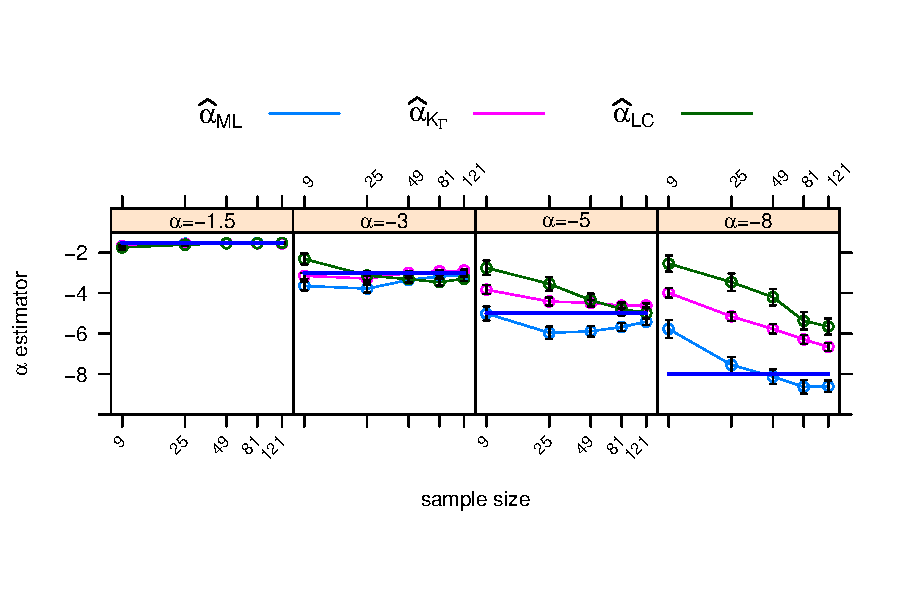
\includegraphics[width=\linewidth]{../../../Figures/OtroPaper/ConGeneraGIAlfaGamma/alfa500_sinmenos20NoCont_MVyNG1yLC_MetAntbarrasdeerror_L3.pdf}
\end{minipage}	
\;	
\begin{minipage}{0.5\linewidth}	
\center{\subsection*{Current methodology}}
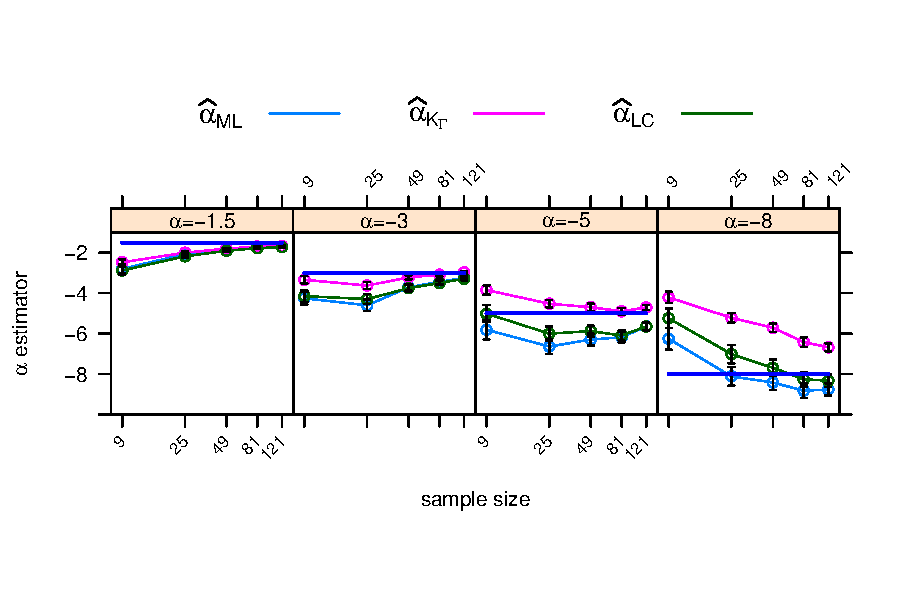
\includegraphics[width=\linewidth]{../../../Figures/OtroPaper/ConGeneraGIAlfaGamma/alfa500_sinmenos20NoCont_MVyNG1yLC_gamma10barrasdeerror_L3.pdf}
\end{minipage}	

\vspace{0.5cm}

\section{Mean Squared Error considering all cases of converge}

\vspace{1cm}

\begin{minipage}{0.5\linewidth}
	\center{\subsubsection*{Previous methodology}}
	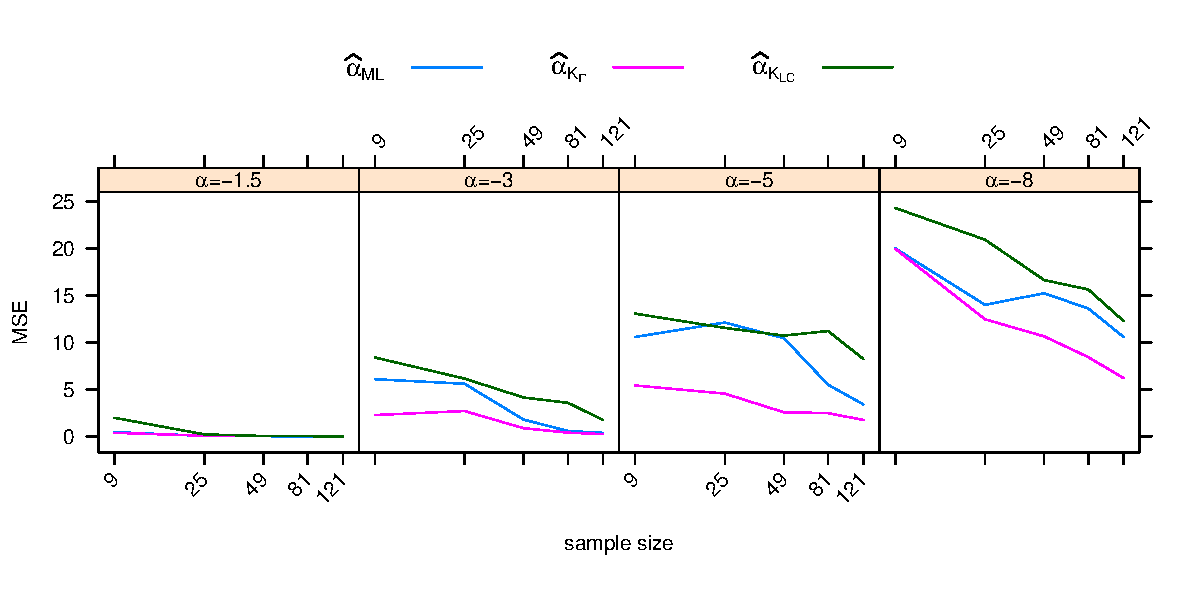
\includegraphics[width=\linewidth]{../../../Figures/OtroPaper/ConGeneraGIAlfaGamma/ECM500_sinmenos20NoCont_MVyNG1yLC_MetAnt_L3.pdf}
\end{minipage}	
\;	
\begin{minipage}{0.5\linewidth}	
	\center{\subsection*{Current methodology}}
	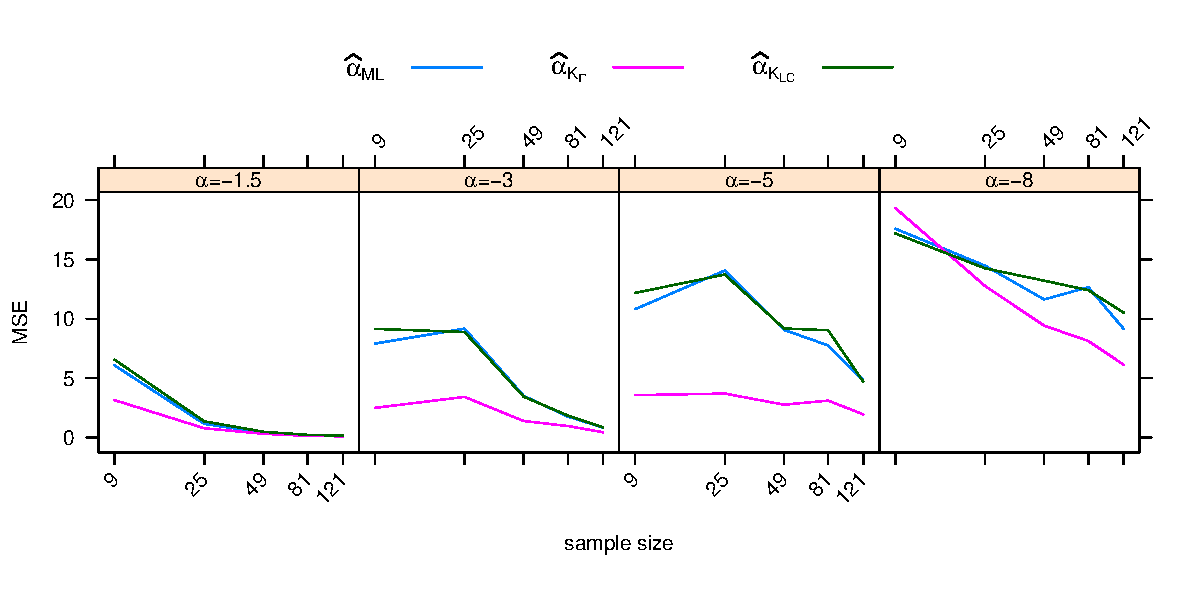
\includegraphics[width=\linewidth]{../../../Figures/OtroPaper/ConGeneraGIAlfaGamma/ECM500_sinmenos20NoCont_MVyNG1yLC_gamma10barrasdeerror_L3.pdf}
\end{minipage}	
\end{document}

